\chapter{Convection at Surface of Lumped Capacitance }
In Lab4 we are going to explore the efficiency of convection on the surface of different solids as we change airflow rate and sample orientations. The principal theories behind this lab have been elaborated in previous notes, and we will review what we have learned so far along the way.
\section{How to be Lumped?}
In a system that transfers heat, we call some parts in the system as "lumped components" whenever their \imp{internal temperature variation is negligible}(i.e., the distribution of temperature is almost uniform). Because of this, we can treat the lumped components as simple thermal resistance/capacitance, which simplifies the analysis of heat transfer process. But how do we know if internal temperature distribution in a subject is uniform enough? 

First we notice that the relative size of lumped components within a heat transfer system matters as we might not be able to ignore what's going on inside a component of a size similar to the whole system. In other words, we need the \imp{characteristic size}\index{characteristic size} of lumped components to be small comparing to the whole system. Second, we learned from our previous experiments that thermal conductivity coefficient affects steepness of temperature profile in medium that transport heat. To see how the thermal conductivity of different materials affects temperature distribution inside material body, let's first imagine a metal rod wrapped in insulating material, and with temperature at its two ends fixed at $T_{end}$. At the middle point, there is a heat source that generates constant heat flux ,$q_{mid}$(see the top schematic in Fig. \ref{fig4-1}). 
\begin{marginfigure}
% Gradient Info
\tikzset {_3b366t10c/.code = {\pgfsetadditionalshadetransform{ \pgftransformshift{\pgfpoint{0 bp } { 0 bp }  }  \pgftransformrotate{0 }  \pgftransformscale{2 }  }}}
\pgfdeclarehorizontalshading{_fyg9w4knt}{150bp}{rgb(0bp)=(0.98,0.72,0.72);
rgb(37.5bp)=(0.98,0.72,0.72);
rgb(49.85119410923549bp)=(1,0.16,0.16);
rgb(62.5bp)=(0.98,0.72,0.72);
rgb(100bp)=(0.98,0.72,0.72)}
\tikzset{every picture/.style={line width=0.75pt}} %set default line width to 0.75pt        
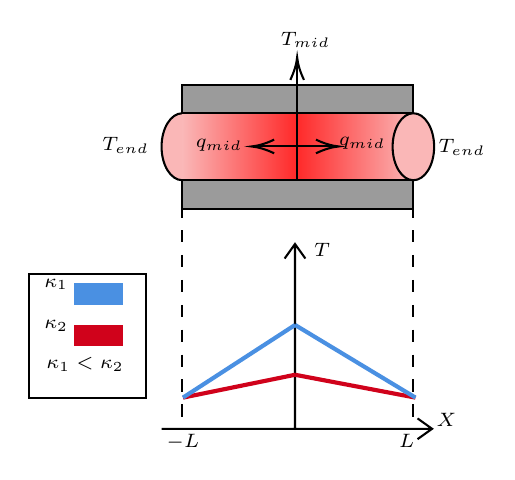
\begin{tikzpicture}[x=0.75pt,y=0.75pt,yscale=-1,xscale=1]
%uncomment if require: \path (0,300); %set diagram left start at 0, and has height of 300

%Shape: Ellipse [id:dp9620775434301283] 
\draw  [fill={rgb, 255:red, 250; green, 183; blue, 183 }  ,fill opacity=1 ] (90,75.87) .. controls (90,66.96) and (94.48,59.73) .. (100,59.73) .. controls (105.52,59.73) and (110,66.96) .. (110,75.87) .. controls (110,84.78) and (105.52,92) .. (100,92) .. controls (94.48,92) and (90,84.78) .. (90,75.87) -- cycle ;
%Shape: Rectangle [id:dp6239956030005828] 
\draw  [draw opacity=0][shading=_fyg9w4knt,_3b366t10c] (100,59.73) -- (211.33,59.73) -- (211.33,91.73) -- (100,91.73) -- cycle ;
%Shape: Rectangle [id:dp08450027404715932] 
\draw  [fill={rgb, 255:red, 155; green, 155; blue, 155 }  ,fill opacity=1 ] (100,46) -- (211.33,46) -- (211.33,59.73) -- (100,59.73) -- cycle ;
%Shape: Rectangle [id:dp030760279476271357] 
\draw  [fill={rgb, 255:red, 155; green, 155; blue, 155 }  ,fill opacity=1 ] (100,92) -- (211.33,92) -- (211.33,105.73) -- (100,105.73) -- cycle ;
%Shape: Ellipse [id:dp6410300181637909] 
\draw  [fill={rgb, 255:red, 250; green, 183; blue, 183 }  ,fill opacity=1 ] (201.33,75.87) .. controls (201.33,66.96) and (205.81,59.73) .. (211.33,59.73) .. controls (216.86,59.73) and (221.33,66.96) .. (221.33,75.87) .. controls (221.33,84.78) and (216.86,92) .. (211.33,92) .. controls (205.81,92) and (201.33,84.78) .. (201.33,75.87) -- cycle ;
%Straight Lines [id:da546691468990532] 
\draw    (155.33,34.73) -- (155.33,91.73) ;
\draw [shift={(155.33,32.73)}, rotate = 90] [color={rgb, 255:red, 0; green, 0; blue, 0 }  ][line width=0.75]    (10.93,-3.29) .. controls (6.95,-1.4) and (3.31,-0.3) .. (0,0) .. controls (3.31,0.3) and (6.95,1.4) .. (10.93,3.29)   ;
%Straight Lines [id:da4067263221168279] 
\draw    (155.67,75.73) -- (173.33,75.73) ;
\draw [shift={(175.33,75.73)}, rotate = 180] [color={rgb, 255:red, 0; green, 0; blue, 0 }  ][line width=0.75]    (10.93,-3.29) .. controls (6.95,-1.4) and (3.31,-0.3) .. (0,0) .. controls (3.31,0.3) and (6.95,1.4) .. (10.93,3.29)   ;
%Straight Lines [id:da5364570928647565] 
\draw    (155.67,75.73) -- (135.33,75.73) ;
\draw [shift={(133.33,75.73)}, rotate = 360] [color={rgb, 255:red, 0; green, 0; blue, 0 }  ][line width=0.75]    (10.93,-3.29) .. controls (6.95,-1.4) and (3.31,-0.3) .. (0,0) .. controls (3.31,0.3) and (6.95,1.4) .. (10.93,3.29)   ;
%Shape: Axis 2D [id:dp26845205848355935] 
\draw  (90,211.76) -- (220.33,211.76)(154.3,122.73) -- (154.3,212) (213.33,206.76) -- (220.33,211.76) -- (213.33,216.76) (149.3,129.73) -- (154.3,122.73) -- (159.3,129.73)  ;
%Straight Lines [id:da10525684167373806] 
\draw [color={rgb, 255:red, 208; green, 2; blue, 27 }  ,draw opacity=1 ][line width=1.5]    (154.33,185.73) -- (100.33,196.73) ;
%Straight Lines [id:da1508811281863801] 
\draw [color={rgb, 255:red, 208; green, 2; blue, 27 }  ,draw opacity=1 ][line width=1.5]    (212.33,196.73) -- (154.33,185.73) ;
%Straight Lines [id:da926366674445905] 
\draw [color={rgb, 255:red, 74; green, 144; blue, 226 }  ,draw opacity=1 ][line width=1.5]    (154.33,161.73) -- (100.33,196.73) ;
%Straight Lines [id:da48496756084972625] 
\draw [color={rgb, 255:red, 74; green, 144; blue, 226 }  ,draw opacity=1 ][line width=1.5]    (154.33,161.73) -- (212.33,196.73) ;
%Straight Lines [id:da9539282308371912] 
\draw  [dash pattern={on 4.5pt off 4.5pt}]  (211.33,92) -- (211.33,211.73) ;
%Straight Lines [id:da5241444385562701] 
\draw  [dash pattern={on 4.5pt off 4.5pt}]  (100,92) -- (100,211.73) ;
%Shape: Rectangle [id:dp7180380607123393] 
\draw  [draw opacity=0][fill={rgb, 255:red, 74; green, 144; blue, 226 }  ,fill opacity=1 ] (48,141.73) -- (71.33,141.73) -- (71.33,152) -- (48,152) -- cycle ;
%Shape: Rectangle [id:dp1387851277373967] 
\draw  [draw opacity=0][fill={rgb, 255:red, 208; green, 2; blue, 27 }  ,fill opacity=1 ] (48,161.73) -- (71.33,161.73) -- (71.33,172) -- (48,172) -- cycle ;
%Shape: Rectangle [id:dp6547879607723921] 
\draw   (26,137) -- (82.33,137) -- (82.33,196.73) -- (26,196.73) -- cycle ;

% Text Node
\draw (146,19) node [anchor=north west][inner sep=0.75pt]  [font=\scriptsize]  {$T_{mid}$};
% Text Node
\draw (222,71) node [anchor=north west][inner sep=0.75pt]  [font=\scriptsize]  {$T_{end}$};
% Text Node
\draw (60,70) node [anchor=north west][inner sep=0.75pt]  [font=\scriptsize]  {$T_{end}$};
% Text Node
\draw (105,70.73) node [anchor=north west][inner sep=0.75pt]  [font=\scriptsize]  {$q_{mid}$};
% Text Node
\draw (174,69.73) node [anchor=north west][inner sep=0.75pt]  [font=\scriptsize]  {$q_{mid}$};
% Text Node
\draw (162,121) node [anchor=north west][inner sep=0.75pt]  [font=\scriptsize]  {$T$};
% Text Node
\draw (221,203) node [anchor=north west][inner sep=0.75pt]  [font=\scriptsize]  {$X$};
% Text Node
\draw (203,213) node [anchor=north west][inner sep=0.75pt]  [font=\scriptsize]  {$L$};
% Text Node
\draw (91,213) node [anchor=north west][inner sep=0.75pt]  [font=\scriptsize]  {$-L$};
% Text Node
\draw (32,138) node [anchor=north west][inner sep=0.75pt]  [font=\scriptsize]  {$\kappa _{1}$};
% Text Node
\draw (32,158) node [anchor=north west][inner sep=0.75pt]  [font=\scriptsize]  {$\kappa _{2}$};
% Text Node
\draw (33,176) node [anchor=north west][inner sep=0.75pt]  [font=\scriptsize]  {$\kappa _{1} < \kappa _{2}$};
\end{tikzpicture}
\caption{A metal rod with fixed end temperature(top), and its steady-state temperature profiles along axial direction(bottom) when it's made of two distinct materials with thermal conductivity coefficient being $\kappa_1$ and $\kappa_2$, respectively.}
\label{fig4-1}
\end{marginfigure}
At the steady state, we ignore temperature variation at radial direction, and obtain a mountain-like temperature profile along the axial direction (see the bottom profiles in Fig.\ref{fig4-1}). With the constant $q_{mid}$, the "steepness" of temperature profile decreases as the thermal conductivity coefficient $\kappa$ increases according to Fourier's law. As a result, the "height" of our mountain will decrease if the rod is made of materials that have larger thermal conductivity coefficient. We thus conclude that to make temperature variation inside heated body negligible, \textbf{the body needs to be highly thermal-conductive.}

\subsection{Biot number}
\imp{Being small and thermal-conductive is \textbf{NOT ENOUGH} for a heated body to be treated as lumped resistance or capacitance}, because so far, we deliberately overlooked the effects of convection at the two ends of the rod in the thought experiment above. Now, if we allow $T_{end}$ to vary by exposing the two ends to an ambient environment. If the ambient temperature $T_{\infty}$ is fixed, then the convective flux at the two ends are $q_{conv}=h(T_{end}-T_{\infty})$, where $h$ is convective heat transfer coefficient. Let $L$ be the distance from the middle point to the rod end. Then, at the steady state, we establish conservation of energy in left(and right) half of the rod as

\begin{equation}
\begin{aligned}
    q_{mid}&=q_{conv}\\
    \kappa\frac{T_{mid}-T_{end}}{L}&=h(T_{end}-T_{\infty})
\end{aligned}
\label{eqn4-1}
\end{equation}
where $T_{mid}$ is the middle-point temperature, and Fourier's Law and Newton's cooling law are used at the second equivalence. If all the temperatures in Eq.(\ref{eqn4-1}) are moved to LHS, we get a dimensionless number at RHS, which is named after the French physicist \textbf{Jean-Baptiste Biot}\footnote{\href{https://en.wikipedia.org/wiki/Jean-Baptiste_Biot}{Biot on Wikipedia}}\index{Biot number}, i.e.,

\begin{equation}
    \frac{T_{mid}-T_{end}}{T_{end}-T_{\infty}}=\frac{hL}{\kappa}.
    \label{eq4-2}
\end{equation}
With the relation in Eq.(\ref{eq4-2}), we are now ready to use \textbf{Biot number} to judge whether a heated body can be treated as a lumped component. Because we require lumped components to have only negligible internal temperature gradient, $T_{mid}-T_{end}$ must be small (i.e. $T_{mid}-T_{end}\approx0$). Since $T_{end}>T_{\infty}$ when the body is heated up, \textbf{the smaller the Biot number is, the more accurate the assumption of lumped component becomes.} A rule of thumb is that we can treat a body as a lumped capacitance/resistance, if its Biot number $Bi=\frac{hL}{\kappa}<0.1$.

\subsection{Nussalt number and thermal conductivity of fluid}
It is not uncommon that people mistake Nussalt number with Biot number, because they have identical expression at first sight. While Biot number can be heuristically understood as a ratio of $\frac{\text{surface convection}}{\text{conduction in solid}}$, Nussalt number\index{Nussalt number} describes heat transfer solely inside the fluid body. Therefore, the thermal conductivity coefficient in Eq.(\ref{eq4-3}) is a property of the fluid in contact with a solid surface.
\begin{equation}
    Nu=\frac{hL}{k_{fluid}}.
    \label{eq4-3}
\end{equation}
A simple derivation of Nussalt number is given as following: Let us imagine a heated solid surface is in contact with a fluid of thickness $L$. When the fluid flows steadily along the surface, the heat flux is then 

\begin{equation}
    q_{conv,fluid}=h(T_s-T_{fluid}),
\end{equation}
where $T_s$ and $T_{fluid}$ are the surface temperature and the temperature of fluid body. If there is no flow, on the other hand, the heat transfers to the fluid through heat conduction only to give
\begin{equation}
    q_{cond,fluid}=k_{fluid}\frac{T_{s}-T_{fluid}}{L}.
\end{equation}
The Nussalt number is then defined as the ratio of $\frac{\text{convection flux}}{\text{conduction flux}}$,i.e.,
\begin{equation}
    Nu=\frac{h(T_s-T_{fluid})}{k_{fluid}\frac{(T_{s}-T_{fluid})}{L}}=\frac{hL}{k_{fluid}}.
\end{equation}

For readers who enjoyed the discussion in Lab2, there is something off regarding the conduction in the fluid. In lab2 we have discussed how the heat flux represented by the flow of electrons is not well-defined at the \textbf{interface between the solid and the ambient environment}, and thus, $q_{conv}=0$ is retained. Within the body of fluid, the conductive flux is, however, well-defined. Instead of having electron flow that carries thermal energy in solid, \imp{the heat conduction in fluid is accomplished by the energy exchange between adjacent molecules.} For a polyatomic molecules\footnote{In fact, it is possible to derive thermal conductivity coefficient from statistically averaged molecular properties, such as mean free path and mean molecular velocities. The methods used for such derivation is under the study of a subject called "statistical mechanics"}, the energy exchange (or collisions) causes changes in vibrational and rotational frequencies, and translational velocities. The table below lists thermal conductivity of some common gases.

\begin{table}[h]
\begin{center}
\tiny
\begin{tabular}{llllllll}
                            &                             & \multicolumn{6}{l}{Thermal conductivity coefficient in $mWm^{-1}K^{-1}$} \\ \hline
\multicolumn{1}{l|}{}       &                             & 100 K      & 200 K      & 300 K      & 400 K     & 500 K     & 600 K     \\ \hline
\multicolumn{1}{l|}{}       & Air                         & 9.5        & 18.5       & 26.4       & 33.5      & 39.9      & 46.0      \\
\multicolumn{1}{l|}{$Ar$}   & Argon (P = 0)               & 6.3        & 12.4       & 17.7       & 22.4      & 26.5      & 30.3      \\
\multicolumn{1}{l|}{$BF_3$} & Boron trifluoride           &            &            & 19.0       & 24.6      &           &           \\
\multicolumn{1}{l|}{$HCl$}  & Hydrogen chloride           &            & 9.2        & 14.5       & 19.5      & 24.0      & 28.1      \\
\multicolumn{1}{l|}{$F_6S$} & Sulfur hexafluoride (P = 0) &            &            & 13.0       & 20.6      & 27.5      & 33.8      \\
\multicolumn{1}{l|}{$H_2$}  & Normal hydrogen (P = 0)     & 68.2       & 132.8      & 186.6      & 230.9     & 270.9     & 309.1     \\
\multicolumn{1}{l|}{$H_2O$} & Water (P=0)                 &            &            & 18.6       & 26.1      & 35.6      & 46.2      \\
\multicolumn{1}{l|}{$D_2O$} & Deuterium oxide (P = 0)     &            &            & 18.2       & 26.6      & 36.3      & 47.6      \\
\multicolumn{1}{l|}{$H_2S$} & Hydrogen sulfide            &            &            & 14.6       & 20.5      & 26.4      & 32.4      \\
\multicolumn{1}{l|}{$H_3N$} & Ammonia                     &            &            & 25.1       & 37.2      & 53.1      & 68.6      \\
\multicolumn{1}{l|}{$He$}   & Helium (P = 0)              & 74.7       & 118.3      & 155.7      & 189.6     & 221.4     & 251.6     \\
\multicolumn{1}{l|}{$Kr$}   & Krypton (P = 0)             &            & 6.5        & 9.5        & 12.3      & 14.8      & 17.1      \\
\multicolumn{1}{l|}{$NO$}   & Nitric oxide                &            & 17.8       & 25.9       & 33.1      & 39.6      & 46.2      \\
\multicolumn{1}{l|}{$N_2$}  & Nitrogen                    & 9.4        & 18.3       & 26.0       & 32.8      & 39.0      & 44.8      \\
\multicolumn{1}{l|}{$N_2O$} & Nitrous oxide               &            & 9.8        & 17.4       & 26.0      & 34.1      & 41.8\\
\hline
\end{tabular}
\caption{\href{https://www.nist.gov/publications/thermal-conductivity-gases}{Tabulated data of thermal conductivity from NIST.} Unless otherwise stated, the measurements are taken under 1 standard atmosphere pressure. The notation "P=0" indicates that the low-pressure limiting value is given.}
\label{tab4-1}
\end{center}
\end{table}

From Table \ref{tab4-1}, we see that the thermal conductivity coefficient of gases increases with temperature. To explain such phenomenon, \imp{it is not sufficient, however, to resort to ideal gas law}\index{ideal gas law},
\begin{equation}
    PV=nRT.
    \label{eq4-7}
\end{equation}
Because most of the data in Table \ref{tab4-1} are obtained with the pressure $P$ fixed at 1 bar, an increase in ambient temperature results in volumetric expansion, reducing the gas number density $\rho=n/V$.\index{number density} Since reduced $\rho$ indicates that gaseous molecule need to travel longer distance before its next collision, the ideal gas law seems to tell us that the rate of molecular energy exchange is quenched at high temperature, resulting decreasing thermal conductivity coefficient.

A heuristic correction to this contradictory explanation lies in the increased kinetic energy of gaseous molecules at high temperature. The excess of kinetic energy promotes the rate of collision despite of the increased distance between molecules, and hence, the rate of energy exchanges is also increased. For readers interested in a more quantitative relationship between temperature and thermal conductivity, a short account of the kinetic theory of monoatomic gas is prepared at the end of current chapter.

\section{Cooling and heating lumped components}
Now that we are persuaded that heated bodied with $Bi<0.1$ are lumped component, it is easy to write down a governing equation, and the solution to it tells transient temperature variation of lumped body over time. Notice that the assumption of lumped component gives us the freedom of ignoring heat conduction inside heated body. So we can establish a conservation of energy by only considering the convection at solid surface, i.e., the thermal energy change in lumped component $\Delta Q$ is solely caused by the convective heat flux $q_{conv}$ on the solid surface of area "$A$". From Eq.(\ref{eq2-3}), we have
\begin{equation}
    \Delta Q=mc_p(T_{init}-T_{body})=q_{conv}Adt,
    \label{eq4-8}
\end{equation}
where $T_{init}$ and $T_{body}$ are initial and current temperature in the lumped component body of interest\footnote{Remember that $c_p$ is specific heat}. Using Newton's cooling law at RHS of Eq.(\ref{eq4-8}) gives
\begin{equation}
    \frac{mc_p(T_{init}-T_{body})}{dt}=hA(T_{body}-T_{\infty})
    \label{eq4-9},
\end{equation}
where the surface temperature is replaced with $T_{body}$ at RHS due to the assumption of lumped body. Now we divide both sides of (\ref{eq4-9}) by $T_{init}-T_{\infty}$ and write LHS as a first-order derivation with respect to time, which results in
\begin{equation}
    -\frac{mc_p}{(T_{init}-T_{\infty})}\frac{dT_{body}}{dt}=hA\frac{T_{body}-T_{\infty}}{T_{init}-T_{\infty}}
    \label{eq4-10}.
\end{equation}
Since $(T_{init}-T_{\infty})$ is a constant, Eq.(\ref{eq4-10}) can be written as an ordinary differential equation (ODE) of the normalized temperature\index{normalized temperature}, $\theta=\frac{T_{body}-T_{\infty}}{T_{init}-T_{\infty}}$, as
\begin{equation}
    -mc_p\frac{d\theta}{dt}=hA\theta
    \label{eq4-11}.
\end{equation}
Eq.(\ref{eq4-11}) has a simple solution of exponential function,i.e.,
\begin{equation}
    \theta=exp\left(-\frac{hA}{mc_p}t\right)=exp(-\alpha t).
    \label{eq4-12}
\end{equation}
Here the constant $\alpha$ (its inverse $\tau=1/\alpha$ is sometimes referred as time constant\index{time constant}) can be further simplified by writing the volume of lumped body, $V$, as a product of its surface area $A$ exposed to fluid, and the inverse of its \imp{\textbf{surface-to-volume ratio}}\index{surface-to-volume ratio} $r_{sv}$ (i.e., $V=A/r_{sv}$). So Eq.(\ref{eq4-12}) becomes
\begin{equation}
    \theta=exp\left(-\frac{hr_{sv}}{\rho_sc_p}t\right)
    \label{eq4-13}
\end{equation}
with $\rho_s$ being the density of lumped component of interest. Eq.(\ref{eq4-13}) sometimes is referred as power-law function\index{power-law function} of lumped component. It clearly shows that the transient temperature variation of lumped components \imp{has nothing to do with the thermal conductivity coefficient.} Instead, the variation is controlled by (1) convective transfer coefficient,(2) surface-to-volume ratio, (3) solid density, and (4) specific heat. \imp{Any action that reduces inverse time constant "$\alpha$" will slow down the cooling process of lumped component.} Fig.\ref{fig4-2} shows that the reduction in $T_{body}$ within first 4 units of time is the most significant when the constant $\alpha$ is the largest.
\begin{marginfigure}
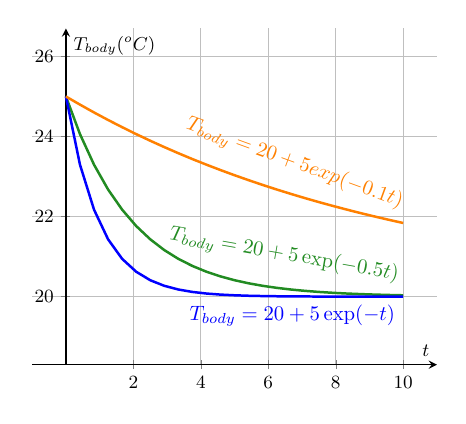
\begin{tikzpicture}[x=0.75pt,y=0.75pt,yscale=0.75,xscale=0.75]
\begin{axis}[grid=both,
          xmax=10,ymax=26,ymin=19,
          axis lines=middle,
          restrict y to domain=0:26,
          restrict x to domain=0:10,
          every axis plot/.append style={very thick},
          xlabel=$t$,
          ylabel=$T_{body}({}^oC)$,
          label style={font=\small},
          tick label style={font=\small},
          enlargelimits]
\addplot[ForestGreen,domain=0:10]  {20+5*exp(-0.5*x)} node[above left,rotate=-10]{$T_{body}=20+5\exp(-0.5t)$};
\addplot[blue,domain=0:10]  {20+5*exp(-x)} node[below left] {$T_{body}=20+5\exp(-t)$};
\addplot[orange,domain=0:10]{20+5*exp(-0.1*x)} node[above left,rotate=-20] {$T_{body}=20+5exp(-0.1t)$};
\end{axis}
\end{tikzpicture}
\caption{Temperature profiles as a function of time "$t$" with $T_{\infty}=20{}^oC$, $T_{init}-T_{\infty}=5{}^oC$, and time constant $\alpha=1$(blue),$0.5$(green), and $0.1$(orange).}
\label{fig4-2}
\end{marginfigure}
The discussion above can be readily applied to the heating process of lumped component. To see this, we write out temperatures explicitly in Eq.(\ref{eq4-13}) as
\begin{equation}
    T_{body}=T_{\infty}+\left(T_{init}-T_{\infty}\right)exp\left(-\frac{hr_{sv}}{\rho_sc_p}t\right).
    \label{eq4-14}
\end{equation}
When the ambient temperature $T_{\infty}$ is higher than the lumped body temperature $T_{body}$, Eq. (\ref{eq4-14}) describes temperature variation of a heating process, and a cooling process otherwise. Fig.\ref{fig4-3} shows that the temperature profiles of a cooling and a heating process are mirror images to each other when $|T_{int}-T_{\infty}|=3^oC$.
\begin{marginfigure}
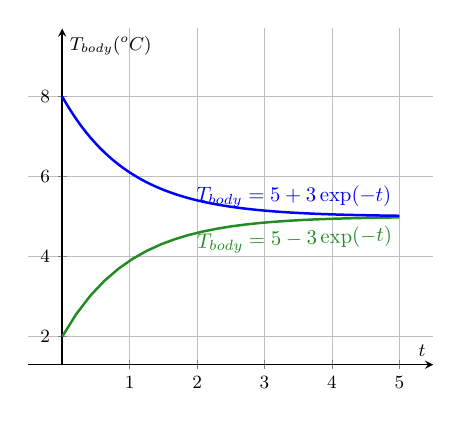
\begin{tikzpicture}[x=0.75pt,y=0.75pt,yscale=0.75,xscale=0.75]
\begin{axis}[grid=both,
          xmax=5,ymax=9,
          axis lines=middle,
          restrict y to domain=0:10,
          restrict x to domain=0:7,
          every axis plot/.append style={very thick},
          xlabel=$t$,
          ylabel=$T_{body}({}^oC)$,
          label style={font=\small},
          tick label style={font=\small},
          enlargelimits]
\addplot[ForestGreen,domain=0:5]  {5-3*exp(-x)} node[below left,rotate=2]{$T_{body}=5-3\exp(-t)$};
\addplot[blue,domain=0:5,samples=100]  {5+3*exp(-x)} node[above left] {$T_{body}=5+3\exp(-t)$};
\end{axis}
\end{tikzpicture}
\caption{Cooling(bottom) and heating(top) process with $|T_{init}-T_{\infty}|=3^oC$ and $T_{\infty}=5^oC$}
\label{fig4-3}
\end{marginfigure}
\subsection{Effects of material properties on convection}
Things become more interesting if we pay extra attention to the four factors in inverse time constant $\alpha$\index{inverse time constant}, and their effects on the cooling/heating rate of lumped component. From Eq. (\ref{eq4-13}), the density $\rho_s$ and the specific heat $c_p$ are two intrinsic material properties, and product of the two varies with material types. The table below lists the values of $\rho_sc_p$ for some common matallic and ceramic materials.
\begin{table}[h]
\small
\begin{tabular}{c|ccc}
\hline
Material & Specific heat(kJ/kgK) & Density(kg/m3) & $c_p\rho_s$ \\ \hline
Aluminum & 0.9                   & 2550           & 2295        \\
Brass    & 0.375                 & 8730           & 3273.75     \\
Stainless steel    & 0.49                  & 8030           & 3934.7      \\
Macor    & 0.79                  & 2520           & 1990.8      \\ \hline
\end{tabular}
\caption{Specific heat and density of some common materials, the data for machinable glass ceramic "Macor" is obtained from \href{https://www.corning.com/worldwide/en/products/advanced-optics/product-materials/specialty-glass-and-glass-ceramics/glass-ceramics/macor.html}{Corning Inc.}}
\label{tab4-2}
\end{table}
If we fix the values of $h$ and $r_{sv}$, Table \ref{tab4-2} shows that steel and Macor have the smallest and the largest inverse time constant $\alpha$, respectively. Starting from the same initial temperature, the rank of cooling/heating rates for these materials follows a sequence of Macor\index{Macor}>Aluminum>Brass>Stainless steel.
\subsection{Effects of geometry of lumped components on convection}
There is no way to fit a decent discussion of the relationship between convective coefficient $h$ with other physical parameters in this note\footnote{Up to March 24th, 2021, there are in total 1,360,000 research papers related to "convective coefficient" available on Google scholar}, which left us with the last factor in $\alpha$: the surface-to-volume ratio, $r_{sv}$. For some highly symmetric shapes, such as sphere and cube, if we assume that the whole lumped body is exposed to convective process, then $r_{sv}$ can be readily calculated by using formula listed in Table \ref{tab4-3}.
\begin{table}[h]
\begin{center}
\small
\begin{tabular}{c|cc}
\hline
Geometry     & Vol.             & $r_{sv}$       \\ \hline
Tetrahedron  & $\sqrt{2}a^3/12$ & ${14.697}/{a}$ \\
Octahedron   & $\sqrt{2}a^3/3$  & ${7.348}/{a}$  \\
Cube         &      $a^3$       & ${6}/{a}$      \\
Sphere       &   $4\pi a^3/3$   & ${3}/{a}$      \\
Dodecahedron &$(15+7\sqrt{5})a^{3}/4$& ${2.694}/{a}$  \\ \hline
\end{tabular}
\end{center}
\caption{$r_{sv}$ of common shapes with $a$ being the length of edge/radius}\
\label{tab4-3}
\end{table}
With these formula, we can also plot $r_{sv}$ against the volumes of these shapes in Fig.\ref{fig4-4}. This simple analysis shows that for a given volume of lumped component, tetrahedron has the largest $r_{sv}$ while sphere has the smallest. Because large $r_{sv}$ results in large $\alpha$, Fig.\ref{fig4-2} and \ref{fig4-4} indicate that \imp{the $T_{body}$ drops(cooling) and increases(heating) much quicker in a tetrahedral component than in a spherical component}. As the lumped body becomes more and more bulky, $r_{sv}$ of all kinds of polyhedral bodies decrease in an order of $O(1/x)$, resulting in more sluggish cooling and heating process. Of course, the bulky component also undermines the validity of lumped capacitance assumption.

\begin{marginfigure}[0in]
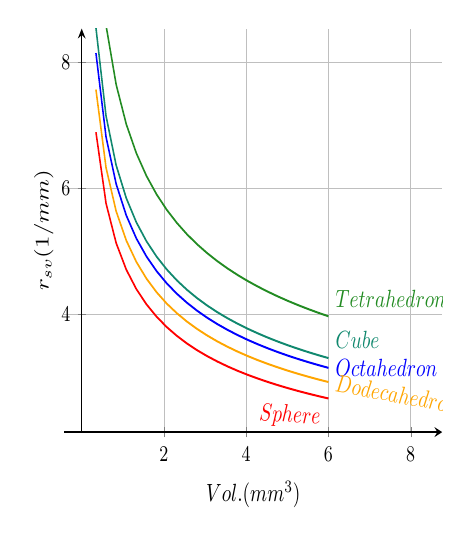
\begin{tikzpicture}[x=0.7pt,y=0.9pt,yscale=0.9,xscale=0.70]
\begin{axis}[grid=both,
          xmax=8,ymax=8,
          axis lines=middle,
          restrict y to domain=0:9,
          restrict x to domain=0:7,
          every axis plot/.append style={ thick},
          xlabel=$Vol.(mm^3)$,
          x label style={at={(axis description cs:0.5,-0.1)},anchor=north},
          y label style={at={(axis description cs:-0.01,.5)},rotate=90,anchor=south},
          ylabel=$r_{sv}(1/mm)$,
          label style={font=\normalsize},
          tick label style={font=\small},
          enlargelimits]
\addplot[ForestGreen,domain=0.1:6]  {14.697/(12*x/sqrt(2))^0.3333} node[above right]{$Tetrahedron$};
\addplot[Blue,domain=0.1:6]  {7.348/(3*x/sqrt(2))^0.3333} node[ right]{$Octahedron$};
\addplot[PineGreen,domain=0.1:6]  {6/(x)^0.3333} node[above right]{$Cube$};
\addplot[red,domain=0.1:6]  {3/(3*x/(4*3.1415926))^0.3333} node[below left,rotate=-3]{$Sphere$};
\addplot[Orange,domain=0.1:6]  {2.694/(4*x/(15+7*sqrt(5)))^0.3333} node[ right,rotate=-8]{$Dodecahedron$};
\end{axis}
\end{tikzpicture}
\caption{$r_{sv}$ versus polyhedral volumes}
\label{fig4-4}
\end{marginfigure}

\section{A kinetic theory for thermal conductivity of gas}
\begin{docspec}
TL;DR: I indulged myself to write this section only because deriving macroscopic law from statistical behavior of molecules is intellectually satisfying. For impatient readers, please check the most important results at the end.
\end{docspec}